% \documentclass[compress, 8pt]{beamer}
\documentclass[handout, 8pt]{beamer}
\usepackage[utf8]{inputenc}

% Notes to self: \nts[color option]{text that is a note}
\newif\ifshowcomments
% \showcommentstrue % uncomment to show
\input{preambleB}

%%%%%%%%%%%%%%%%%%%%%%%%%%%%%%%%%%%%%%%%%%%%%%%%%%%%%%%%%%%%%%%%%%%%%%%%%%%%%%
% Paths to figures
\newcommand{\orange}[1]{\textbf{\color{Orange}#1}}

\newcommand{\model}{/Users/tarasullivan/Documents/dissertation/model/fig_tex_code}

% \newcommand{\nn}[2][DarkGray]{{\small \color{#1} #2}}
% \newcommand{\ccdoi}[2]{\href{https://doi.org/#1}{\nn{#2}}}

% Avoid a warning on mac; can introduce a warning (and maybe a break) on windows
% \usepackage{etex}
% Avoid a warning
\let\Tiny=\tiny

%Information to be included in the title page:
\title{ECON726: Policy and Program Evaluation}
\author[]{Tara Sullivan}
\institute{
% Macro Lunch Presentation \\
Tara Sullivan \\
\textit{tara.sullivan55@login.cuny.edu}
}
\date{
\today
\nts{\\
\medskip
Notes/comments are in gray and will be excluded from the presentation.
}
}

% plot graphs with pgfplots
\usepackage{pgfplots}
\pgfplotsset{compat=newest}
\usepgfplotslibrary{groupplots}
\usepgfplotslibrary{dateplot}
\pgfplotsset{compat=newest,
    every axis/.style={
        axis y line*=left,
        axis x line*=bottom,
        % allows for multi-line legend entries
        legend style={cells={align=left}},
        % allows for multi-line titles
        title style={align=center},
    },
}

% % path to tex images
% \makeatletter
% \def\input@path{{../../img/}}
% \makeatother

%% Use tikzset instead of tikzstyle which is deprecated
% \tikzset{line/.style = {draw, -latex'},
%         cloud/.style = {draw, ellipse, node distance=3cm,
%                         minimum height=2em}}

% \tikzset{var/.style = {
% draw, circle, %minimum size=1cm,
% % inner sep=0pt
% }}

% For animations using underbrace 
% Source: https://tex.stackexchange.com/a/565866
\usepackage{xparse, letltxmacro}
\LetLtxMacro{\oldunderbrace}{\underbrace}
\DeclareDocumentCommand{\underbrace}{d<> m e{_}}{%
  \IfValueTF{#1}{% IF <overlay-specification> given
    % using global onlside flag, cf. p82 beamer manual v3.59
    \oldunderbrace{#2\onslide<#1>}_{#3}\onslide%
  }{% ELSE
    \oldunderbrace{#2}_{#3}
  }%
}%

%%%%%%%%%%%%%%%%%%%%%%%%%%%%%%%%%%%%%%%%%%%%%%%%%%%%%%%%%%%%%%%%%%%%%%%%%%%%%%%%
\begin{document}    
%\beamertemplatenavigationsymbolsempty


%%%%%%%%%%%%%%%%%%%%%%%%%%%%%%%%%%%%%%%%%%%%%%%%%%%%%%%%%%%%%%%%%%%%%%%%%%%%%%%%
\begin{frame}
\titlepage
% \tikzset{external/figure name={intro_}}
\end{frame}

%%%%%%%%%%%%%%%%%%%%%%%%%%%%%%%%%%%%%%%%%%%%%%%%%%%%%%%%%%%%%%%%%%%%%%%%%%%%%%%
\miniframesoff
\begin{frame}{Outline}
    \tableofcontents
\end{frame}
\miniframeson

%%%%%%%%%%%%%%%%%%%%%%%%%%%%%%%%%%%%%%%%%%%%%%%%%%%%%%%%%%%%%%%%%%%%%%%%%%%%%%%%
\section[Overview]{Course Overview}

% \input{01-intro}
%%%%%%%%%%%%%%%%%%%%%%%%%%%%%%%%%%%%%%%%%%%%%%%%%%%%%%%%%%%%%%%%%%%%%%%%%%%%%%%%
\begin{frame}{Course overview}

\textbf{Description:} In real-world settings, analysts must draw inferences about causes and effects from observational, i.e., non-randomized, data. For example, 

\begin{itemize}

\item How do we truly determine whether charter schools produce better student outcomes?

\item Whether a marketing campaign has increased consumer awareness? 

\end{itemize}


\vspace{2em}
This course will cover statistical methods for \textbf{causal inference} to help analysts design and analyze observational studies, for real-world decision-making. 

\vspace{2em}
\pause
\textbf{Informal goal:}
\begin{itemize}
    \item Understand the tenants of causal inference
    \item Challenge yourself to learn a new methodology well
    \item Learn some basic python
    \item Communicate results effectively
\end{itemize}


\end{frame}

%%%%%%%%%%%%%%%%%%%%%%%%%%%%%%%%%%%%%%%%%%%%%%%%%%%%%%%%%%%%%%%%%%%%%%%%%%%%%%%%
\begin{frame}{Prerequisites}

\begin{itemize}

    \item This is a course in econometrics and applied statistics; as such, it is expected that you have a strong interest in business and public policy applications


\vspace{1em}
\item You are required to have taken a semester-long course in probability and statistical inference 

\begin{itemize}
    \item Ideally, you have completed coursework in regression methods; otherwise, the econometric theory and the technical approach for the course will be difficult to follow
\end{itemize}

\pause
\vspace{1em}
\item Statistical analysis software is the primary tool for this course, and I will be providing course instructions in \textbf{python}. 
\begin{itemize}
    \item You will be expected to complete course assignments in python*
\end{itemize}

\end{itemize}

\end{frame}

%%%%%%%%%%%%%%%%%%%%%%%%%%%%%%%%%%%%%%%%%%%%%%%%%%%%%%%%%%%%%%%%%%%%%%%%%%%%%%%%
\begin{frame}{Grading}

\begin{itemize}
    \item Empirical project: 75\% of final grade


    \vspace{2em}
    \item Homework/quizzes: 15\% of final grade

    \vspace{2em}
    \item Attendance and participation: 10\% of final grade
\end{itemize}

\end{frame}

%%%%%%%%%%%%%%%%%%%%%%%%%%%%%%%%%%%%%%%%%%%%%%%%%%%%%%%%%%%%%%%%%%%%%%%%%%%%%%%%
\begin{frame}{Empirical project}

The project is based on an empirical paper of your choice which:
\begin{enumerate}
     \item Uses a method discussed in this course*
     \item Has data available online
     \item Is not based on an experiment*
 \end{enumerate} 
 

\vspace{2ex}
The paper should:
\begin{enumerate}
    \item Be based on a paper published in a peer-reviewed journal
    \item Briefly state the research question and discuss the dataset 
    \item Provide a (formal) discussion of the identification strategy (What is the ideal randomized experiment? What sort of bias would na{\"i}ve  approaches introduce? Why is this methodology causal?)
    \item Replicate (selected) main findings
    \item Describe and implement some sort of extension to this paper. This could be new and interesting tests for key assumptions, robustness checks, additional results based on other methods or data, or combination thereof
\end{enumerate}

\end{frame}

%%%%%%%%%%%%%%%%%%%%%%%%%%%%%%%%%%%%%%%%%%%%%%%%%%%%%%%%%%%%%%%%%%%%%%%%%%%%%%%%
\begin{frame}{}

\textbf{Paper selection}: Due \textbf{September 16} [5\% of final grade]
\begin{itemize}
\item Select your paper. Briefly describe the causal effect of interest and methodology. Discuss what you think you will do for your extension of this paper. 
\end{itemize}

\textbf{Project plan}: Due \textbf{October 14} [15\% of final grade] 
\begin{itemize}
\item This paper should be your first effort at addressing points (1) and (2) above. 
Summarize the public policy or business context of the paper. 
Write down the specific question the paper is evaluating.
Discuss the data your are using (both your replication data, and data for your extension)
Discuss the extensions you are considering, and, if necessary, where you will be getting that data. 
\end{itemize} 

\textbf{Replication results}: Due \textbf{November 4}: [10\% of final grade]
\begin{itemize}
\item You should submit some of your main replication results. The final results should be formatted as tables and charts in a word document or PDF, submitted on Brightspace. Your code and data should accessible on GitHub.
\end{itemize}

\textbf{Presentation}: Due \textbf{December 2} \& \textbf{December 9} [10\% of final grade]
\begin{itemize}
\item Prepare a 5-10 minute presentation on your paper. Focus on the research question, main result, and one extension. 
\end{itemize}

\textbf{Final Paper}: Due \textbf{December 16} [35\% of final grade]
\begin{itemize}
\item Your paper should contain 5-8 pages of text, and 5-8 pages of figures (double spaced, 12 point font).
You are expected to use python, and must provide the code and data to replicate your findings. 
Your final project should be submitted on Brightspace, and your code and data should be uploaded to github (note: if your data is too large to upload to github, let me know). 
\end{itemize}

\end{frame}

%%%%%%%%%%%%%%%%%%%%%%%%%%%%%%%%%%%%%%%%%%%%%%%%%%%%%%%%%%%%%%%%%%%%%%%%%%%%%%%%
\begin{frame}{Selecting a paper}

Top 5 economics journals:
\begin{itemize}
    \item American Economic Review
    \item Econometrica
    \item Journal of Political Economy
    \item Quarterly Journal of Economics
    \item Review of Economic Studies
\end{itemize}
Also good:
\begin{itemize}
    \item American Economic Journal: Applied Economics
    \item Journal of Public Economics
    \item Review of Economics and Statistics
\end{itemize}
% Here is a random list online of good [economics] journals: \url{https://www.stern.nyu.edu/sites/default/files/assets/documents/Econ%20Top%20Journals%20-%20July%202020.pdf}


Data used in the Mostly Harmless Econometrics book: \url{https://economics.mit.edu/people/faculty/josh-angrist/mhe-data-archive}
\begin{itemize}
    \item Note that Krueger (1999) is based on an experiment, and would not be appropriate for this assignment
\end{itemize}

\end{frame}




%%%%%%%%%%%%%%%%%%%%%%%%%%%%%%%%%%%%%%%%%%%%%%%%%%%%%%%%%%%%%%%%%%%%%%%%%%%%%%%%
\begin{frame}{AI Policy}

\begin{itemize}
\item This course is mean to extend your theoretical and empirical abilities. 
Over-reliance on LLMs will hamper that effort. 
Overall, my aim is to reward genuine effort, over seemingly perfect code and text. 
\item To that end, I highly encourage you to avoid AI for your work. 
I understand it may be helpful for brainstorming and troubleshooting, but please ensure that your written code and words are your own. 

\item To be transparent about my AI usage: I will primarily use LLMs to brainstorm and troubleshoot. 
I've been advised by other professors to run your code through AI for grading purposes (as a secondary grader); if you would prefer I don't do that, please don't hesitate to let me know. 

\item Overall, this policy is meant to be a dialogue, not dogma. 
Please feel free to let me know your thoughts. 

\end{itemize}

\end{frame}



%%%%%%%%%%%%%%%%%%%%%%%%%%%%%%%%%%%%%%%%%%%%%%%%%%%%%%%%%%%%%%%%%%%%%%%%%%%%%%%%
\begin{frame}{Course outline}

\textbf{Outline}
\begin{enumerate}
\item Introduction/idealized experiment

% \begin{itemize}
% \item Reading: \textcite{AP09}, Chapter 1
% \item Homework: Download python. Run some python code. Set up a GitHub repository, and send me your code (you can either add me as a collaborator, or make your repository poublic).
% \end{itemize}

%2. 
\item Probability and Statistics review

%
\item Potential outcomes and experiments

% \begin{itemize}
% \item Reading: \textcite{AP09}, Chapter 2
% \end{itemize}

\item Linear regression models 
% \begin{itemize}
% \item Reading: \textcite{AP09}, Chapter 3
% \end{itemize}

\item Matching and Propensity models
% \begin{itemize}
% \item Reading: \textcite{AP09}, Chapter 3
% \end{itemize}

\item Difference-in-differences models

\item Synthetic Control

\item Machine learning methods in Causal inference

\end{enumerate}

\vspace{2ex}
Currently not listed: instrumental variables
\begin{itemize}
    \item Currently not discussing instrumental variables (Angrist and Pischke 2009, Chapter 4)
    \item This can be a topic you explore in your empirical project
\end{itemize}

\end{frame}

%%%%%%%%%%%%%%%%%%%%%%%%%%%%%%%%%%%%%%%%%%%%%%%%%%%%%%%%%%%%%%%%%%%%%%%%%%%%%%%%
\begin{frame}{Resources}

The primary textbook for this course is \textbf{Mostly Harmless Econometrics} (Angrist and Pischke, 2009).
This textbook is meant to provide a readable introduction to many topics of this course. 
It is available though the Hunter College bookstore (\href{https://hunter.textbookx.com/institutional/index.php?action=browse\#books/4891202/}{link}), though is cheaper on Amazon 

\vspace{2ex}
A number of other resources exist on this topic:

\vspace{1ex}
\textbf{Causal Inference for the Brave and True} (Alves 2022)
\begin{itemize}
\item Excellent \href{https://matheusfacure.github.io/python-causality-handbook/landing-page.html}{online} companion to Mostly Harmless; I will cite from this website throughout the course. Effectively brings the methods from Mostly Harmless into the machine learning age, with sample code in Python. Be aware there are (very occasional!) errors.
\end{itemize}

\vspace{1ex}
\textbf{Business Data Science} (Taddy 2019) %\parencite{T19}
\begin{itemize}
\item Sometimes called the ``machine learning Mostly Harmless.'' I will borrow heavily from Chapters 5 (Experiments) and 6 (Controls). Note that the code provided in the book is written in R. 
\end{itemize}

\vspace{1ex}
\textbf{Applied Causal Inference Powered by ML and AI} (Chernozhukov et al. 2025)
\begin{itemize}
\item Covers similar topics as Mostly Harmless, but from an ML perspective. Currently available free \href{https://causalml-book.org/}{online}. 
\end{itemize}

\end{frame}


%%%%%%%%%%%%%%%%%%%%%%%%%%%%%%%%%%%%%%%%%%%%%%%%%%%%%%%%%%%%%%%%%%%%%%%%%%%%%%%
% \miniframesoff
\section[Intro Causal Inference]{Introduction to Causal Inference and Randomization}
\miniframesoff
\begin{frame}
    \tableofcontents[currentsection]
\end{frame}
\miniframeson

%%%%%%%%%%%%%%%%%%%%%%%%%%%%%%%%%%%%%%%%%%%%%%%%%%%%%%%%%%%%%%%%%%%%%%%%%%%%%%%%
\begin{frame}{Causal questions}


\begin{figure}
\begin{tikzpicture}
\node [draw, circle] (X) {X};
\node [draw, circle, right =of X] (Y) {Y};
\draw (X) edge[->] (Y);
\end{tikzpicture}
\end{figure}

\vspace{2ex}
Does $X$ cause $Y$?

\pause
\vspace{2ex}
If $X$ causes $Y$, how large is the effect of $X$ on $Y$?

\pause
\vspace{2ex}
Is the size of this effect large relative to the effects of other causes of $Y$?

\pause
\vspace{2ex}
If individuals with $X = x^\prime$ instead had $X = x^{\prime\prime}$, how much would their value of $Y$ change?

\pause
\vspace{2ex}
\textbf{Examples of applied questions:}
\begin{itemize}
    \item What is the effect of class size on test scores?
    \item What is the effect of training programs on re-employment?
    \item How does schooling affect future earnings?
\end{itemize}
Examples of other causal questions?

\end{frame}

%%%%%%%%%%%%%%%%%%%%%%%%%%%%%%%%%%%%%%%%%%%%%%%%%%%%%%%%%%%%%%%%%%%%%%%%%%%%%%%%
\begin{frame}{Example: Effect of hospital visits on health}

Suppose you want to know the effect of hospital visits on health. To that end, you look at some data on self-assessed health and hospital stays.
\pause
\begin{table}
\begin{tabular}{ll}
$Y$ & An individual's self-assessed health \\
$D \in \{0, 1\}$ & 1 if they stayed in the hospital in the past 12 months; 0 otherwise
\end{tabular}
\end{table}

\begin{table}
\begin{tabular}{cccc}
Group &$N$  &$\bar{Y}$  &$\hat{\sigma}$  \\
&(sample size) &(sample mean) &(standard error) \\
\hline
$D=1$ &7,774 &3.21 &0.0014 \\
$D=0$ &90,049 &3.93 &0.003 \\
\end{tabular}
\end{table}

\pause
\vspace{2ex}
What if we compare the health of those admitted to the hospital to the health of those who weren't?
\begin{equation*}
\bar{Y}_1 - \bar{Y}_0 = 3.21 - 3.93 = -0.72
\end{equation*}
\pause
On average, the health of people who stayed in a hospital is \textbf{lower}

\vspace{1ex}
\textbf{Do hospitals cause bad health?}
\end{frame}

%%%%%%%%%%%%%%%%%%%%%%%%%%%%%%%%%%%%%%%%%%%%%%%%%%%%%%%%%%%%%%%%%%%%%%%%%%%%%%%%
\begin{frame}{Potential Outcomes framework}

The question is whether $Y$ is \textbf{affected} by hospital care. 
A helpful framework for thinking about these problems is the \textbf{potential outcomes framework}
 
\begin{table}
\begin{tabular}{ll}
$D_i \in \{0, 1\}$ &Binary treatment variable for individual $i$ \\ 
$Y_i$ &Measure of health status for individual $i$\\
\pause
$Y_{1i}$ &Health outcome if individual $i$ stays in the hospital ($D_i=1$) \\
&Alternative notation: $Y_i(1)$, $Y_i^1$, $y_{i1}$ \\
$Y_{0i}$ &Health outcome if individual $i$ stays in the hospital ($D_i=0$)  \\
&Alternative notation: $Y_i(0)$, $Y_i^0$, $y_{i0}$ \\\\
\end{tabular}
\end{table}

\begin{itemize}
    \item $Y_{0i}$ is the health status of an individual had they not gone to the hospital, \emph{irrespective of whether they actually went}
    \item Causal effect of hospitalization for individual $i$ is the difference $Y_{1i} - Y_{0i}$
\end{itemize}

\pause
\vspace{2ex}
Observed outcome $Y_i$ can be written as:
\begin{align*}
    Y_i =& \begin{cases}
    Y_{1i} &\text{if} D_i = 1 \\
    Y_{0i} &\text{if} D_i = 0
    \end{cases} \\
    =& Y_{0i} + (Y_{1i} - Y_{0i}) D_i
\end{align*}
\end{frame}


%%%%%%%%%%%%%%%%%%%%%%%%%%%%%%%%%%%%%%%%%%%%%%%%%%%%%%%%%%%%%%%%%%%%%%%%%%%%%%%%
\begin{frame}{Fundamental problem of causal inference}

\begin{columns}

\column{0.75\linewidth}

\textbf{Problem:}
\begin{itemize}
    \item If an individual is treated ($D_i = 1$), we never observe the outcome in which they are not treated ($Y_{i0}$)
    \item If an individual is not treated ($D_i = 0$), we never observe the outcome in which they are treated ($Y_{1i}$)
\end{itemize}

\vspace{2ex}
\textbf{\color{HunterPurple} The causal effect $\mathbf{Y_1 - Y_0}$ is unidentifiable}

\begin{table}
\begin{tabular}{lll}
Group &$Y_1$ &$Y_0$ \\
$D = 1$ &Observable as $Y$ &Unobservable counterfactual \\
$D = 0$ &Unobservable counterfactual &Observable as $Y$
\end{tabular}
\end{table}

\pause
\column{0.25\linewidth}
\begin{figure}
% \input{img/potential_outcomes.tex}
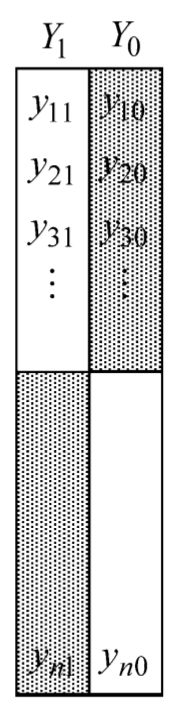
\includegraphics[height=2in]{img/potential_outcomes.png}
\end{figure}

\end{columns}

\end{frame}

%%%%%%%%%%%%%%%%%%%%%%%%%%%%%%%%%%%%%%%%%%%%%%%%%%%%%%%%%%%%%%%%%%%%%%%%%%%%%%%%
\begin{frame}{Na{\"i}ve comparison: $\EE [Y \vert D = 1] - \EE [Y \vert D=0]$}

 Recall that:
\begin{itemize}
    \item The expectations operator $\EE [\cdot]$ is the average of a random variable
    \item The conditional expectations operator $\EE [\cdot \vert \cdot]$ takes the average over particular values. So $\EE [Y \vert D=1]$ is the average value of $Y$ when for observations where $D = 1$
    \item The math symbol for ``because'' is $\because$
    \item We can drop the individual subscript $i$ for convenience
\end{itemize}

\vspace{2ex}
Let's consider the averages of $Y_{1i}$, $Y_{0i}$, and $Y_i$:
\begin{align*}
\EE [ Y \vert D = 1 ] =& \EE [Y_0 + (Y_1 - Y_0) D \vert D = 1]
&&\because Y = Y_0 + (Y_1 - Y_0) D \\
=& \alert<3>{\EE[Y_1 \vert D = 1]}\\
\EE[Y \vert D = 0] 
% =& E [Y_0 + (Y_1 - Y_0) D \vert D = 0] \\
=& \alert<3>{\EE[Y_0 \vert D = 0]}
\end{align*}

\vspace{2ex}

\onslide<2->
We can re-write the observed difference in health outcomes as:
\begin{align*}
\onslide<3->{\EE [Y \vert D = 1] - \EE [Y \vert D=0] 
=& \alert<3>{\EE [Y_1 \vert D=1]} - \alert<3>{\EE [Y_0 \vert D=0]} \\}
\onslide<4->{=& \EE [Y_1 \vert D=1] \alert<4>{- \EE [Y_0 \vert D = 1] + \EE [Y_0 \vert D = 1]}  - \EE [Y_0 \vert D=0] \\}
\onslide<5->{=& \underbrace<6->{\EE [Y_1 - Y_0 \vert D = 1]}_{\text{Avg. treatment effect on treated}} 
\onslide<5->{+} \underbrace<6->{\EE [Y_0 \vert D = 1] - \EE [Y_0 \vert D=0]}_{\text{Selection bias}}}
\end{align*}

\end{frame}

%%%%%%%%%%%%%%%%%%%%%%%%%%%%%%%%%%%%%%%%%%%%%%%%%%%%%%%%%%%%%%%%%%%%%%%%%%%%%%%%
\begin{frame}{Na{\"i}ve comparison (cont.)}

Observed difference in health outcomes equals the average treatment effect (ATE) on the treated plus selection bias:
\begin{align*}
\EE [Y \vert D = 1] - \EE [Y \vert D=0] 
% =& \EE [Y_1 \vert D=1] { - \EE [Y_0 \vert D = 1] + \EE [Y_0 \vert D = 1]}  - \EE [Y_0 \vert D=0] \\
=& \underbrace{\EE [Y_1 - Y_0 \vert D = 1]}_{\text{ATE on treated}} 
+ \underbrace{\EE [Y_0 \vert D = 1] - \EE [Y_0 \vert D=0]}_{\text{Selection bias}}
\end{align*}
ATE on treated is the average causal effect of hospitalization on those who were hospitalized:
\begin{equation*}
    \EE [Y_1 \vert D=1] - \EE [Y_0 \vert D = 1] = \EE [Y_1 - Y_0 \vert D = 1]
\end{equation*}
Selection bias:
\begin{equation*}
    \EE [Y_0 \vert D = 1] - \EE [Y_0 \vert D=0]
\end{equation*}
\textbf{What do you think selection bias looks like in this example?}

\pause
\begin{itemize}
    \item The difference in $Y_{0i}$ between those who were and were not hospitalized
    \item The sick are more likely than the healthy to be hospitalized
    \begin{itemize}
        \item[$\implies$] Those who were hospitalized have worse values of $Y_{0i}$

        \item[$\implies$] Selection bias is negative
    \end{itemize}
\end{itemize}
\end{frame}


%%%%%%%%%%%%%%%%%%%%%%%%%%%%%%%%%%%%%%%%%%%%%%%%%%%%%%%%%%%%%%%%%%%%%%%%%%%%%%%%
\begin{frame}{Random assignment and selection bias}

Random assignment will solve the selection problem! 

\vspace{2ex}
Assume potential outcomes are independent of the treatment ($Y_0, Y_1 \perp D$):
\begin{align*}
    \implies&
    \EE [Y_1 \vert D] = \EE [Y_1] \quad\quad
    \text{and} \quad\quad \EE [Y_0 \vert D] = \EE [Y_0] \\
    \implies&
    \EE [Y_1 \vert D] = \EE [Y_0 \vert D] \\
    \implies&
    \EE [Y_1 \vert D] - \EE [Y_0 \vert D] = 0 \\
    \implies&
    \text{Selection bias is 0} \\
    \implies&
    \text{Na{\"i}ve comparison = ATE on treated}
\end{align*}
$\implies$ Randomization makes treatment and control comparable.

\vspace{2ex}
Na{\"i}ve comparison under randomization:
\begin{align*}
    \EE [Y \vert D = 1] - \EE [Y \vert D=0]  
    =& \EE [Y_1 \vert D = 1] - \EE [Y_0 \vert D = 0] \\
    =& \EE [Y_1 \vert D = 1] - \EE [Y_0 \vert D = 1] \\
    =& \EE [Y_1 - Y_0 \vert D = 1] \\
    =& \EE [Y_1 - Y_0] \\
    =& \EE [Y_1] - \EE [Y_0]
    % =& \EE [Y_1 - Y_0 \vert D = 1] + \EE [Y_0 \vert D = 1] - \EE [Y_0 \vert D=0] \\
    % =& \EE [Y_1 - Y_0 \vert D = 1] \\
    % =& \EE [Y_1 \vert D = 1]
\end{align*}
Randomization $\implies$ ATE on treated equals ATE


\end{frame}


%%%%%%%%%%%%%%%%%%%%%%%%%%%%%%%%%%%%%%%%%%%%%%%%%%%%%%%%%%%%%%%%%%%%%%%%%%%%%%%%
\begin{frame}{Randomization}

Randomization makes treatment and control groups comparable
\begin{itemize}
    \item This is why randomization is often considered the ``gold standard in causal analysis''
\end{itemize}

\vspace{2ex}
Randomization is hard in practice!
\begin{itemize}
    \item Randomization does hold in the hospitalization example
    \item How could you test whether randomization holds?

\end{itemize}

\vspace{2ex}
In this class we will discuss:
\begin{itemize}
    \item Importance of randomization from a theoretical perspective
    \item What to do when randomization does not hold
\end{itemize}

\end{frame}

%%%%%%%%%%%%%%%%%%%%%%%%%%%%%%%%%%%%%%%%%%%%%%%%%%%%%%%%%%%%%%%%%%%%%%%%%%%%%%%%
\begin{frame}{Optional - Randomization and regression}

Assume treatment effects are constant and the same for everyone
\begin{align*}
    Y_i =& Y_{0i} + (Y_{1i} - Y_{0i}) D_i \\
    \onslide<2->{=& 
    {\color{HunterPurple} \EE [Y_{0i}]}
    + (Y_{1i} - Y_{0i}) D_i 
    + Y_{0i} {\color{HunterPurple} - \EE [Y_{0i}]} \\}
    \onslide<3->{
    =& 
    \underbrace{\EE [Y_{0i}]}_{\alpha}
    + \underbrace{(Y_{1i} - Y_{0i})}_{\beta} D_i 
    + \underbrace{Y_{0i} - \EE [Y_{0i}]}_{\eta_i \text{ (Random part of $Y_{0i}$)}} \\}
    \onslide<4->{
    =& \alpha + \beta D_i + \eta_i}
\end{align*}

\onslide<5->
Evaluate this with the treatment on ($D = 1$) and off ($D = 0$):
\begin{align*}
    D = 1 \implies \EE [Y \vert D = 1] 
    &= \alpha + \beta + \EE [\eta \vert D = 1] \\
    D = 0 \implies \EE [Y \vert D = 0] 
    &= \alpha + \EE [\eta \vert D = 0] \\
\end{align*}


\onslide<6->
Then: 
\begin{align*}
    \EE [Y \vert D = 1] - \EE [Y \vert D = 0] 
    =& (\alpha + \beta + \EE [\eta \vert D = 1]) - (\alpha + \EE [\eta \vert D = 0]) \\
    =& \beta + \underbrace{(\EE [\eta \vert D = 1] - \EE [\eta \vert D = 0])}_{\text{selection bias}}
\end{align*}

\onslide<7->
Selection bias will equal zero if the correlation between the error term and treatment assignment is zero. 
\begin{itemize}
    \item If $D$ is randomly assigned, regression of $Y$ onto $D$ (and a constant) yields the causal effect $\beta$
\end{itemize}


\end{frame}

%%%%%%%%%%%%%%%%%%%%%%%%%%%%%%%%%%%%%%%%%%%%%%%%%%%%%%%%%%%%%%%%%%%%%%%%%%%%%%%%
\begin{frame}{Homework}

Homework due next week (on Brightspace)
\begin{itemize}
    \item Create a GitHub account (you can use a student account)
\end{itemize}

Things you should be working towards:
\begin{itemize}
    \item Order Angrist and Pischke (2009); Chapter 1 \& 2 (in 2 weeks)
    \item Consider which paper you would like to base your empirical project on (due in 2 weeks)
    \begin{itemize}
        \item \textbf{Note:} something you should do in your written analysis is consider what the ideal experiment looks like, and what the selection bias in outcomes is
    \end{itemize}
    
\end{itemize}

\end{frame}





% %%%%%%%%%%%%%%%%%%%%%%%%%%%%%%%%%%%%%%%%%%%%%%%%%%%%%%%%%%%%%%%%%%%%%%%%%%%%%%%
% \miniframesoff
% \section[C2: Model]{Chapter 2: Model}
% \begin{frame}
%     \tableofcontents[currentsection]
% \end{frame}
% \miniframeson

% \input{c2-02-model}

% %%%%%%%%%%%%%%%%%%%%%%%%%%%%%%%%%%%%%%%%%%%%%%%%%%%%%%%%%%%%%%%%%%%%%%%%%%%%%%%
% \miniframesoff
% \section[C2: Simulations]{Chapter 2: Simulations}
% \begin{frame}
%     \tableofcontents[currentsection]
% \end{frame}
% \miniframeson

% \input{c2-03-sims.tex}

% %%%%%%%%%%%%%%%%%%%%%%%%%%%%%%%%%%%%%%%%%%%%%%%%%%%%%%%%%%%%%%%%%%%%%%%%%%%%%%%
% \tikzset{external/figure name={data_}}
% \miniframesoff
% \section[C1: Intro]{Chapter 1: Introduction}
% \begin{frame}
%     \tableofcontents[currentsection]
% \end{frame}
% \miniframeson

% \input{c1-01-intro}


% %%%%%%%%%%%%%%%%%%%%%%%%%%%%%%%%%%%%%%%%%%%%%%%%%%%%%%%%%%%%%%%%%%%%%%%%%%%%%%%
% \miniframesoff

% \section[C1: Data]{Chapter 1: Overview of data}
% \begin{frame}
%     \tableofcontents[currentsection]
% \end{frame}
% \miniframeson

% \input{c1-02-data}

% %%%%%%%%%%%%%%%%%%%%%%%%%%%%%%%%%%%%%%%%%%%%%%%%%%%%%%%%%%%%%%%%%%%%%%%%%%%%%%%
% \miniframesoff
% \section[C1: Outcomes]{Chapter 1: Switching and graduation outcomes}
% \begin{frame}
%     \tableofcontents[currentsection]
% \end{frame}
% \miniframeson

% \input{c1-03-grad_outcomes}
% %%%%%%%%%%%%%%%%%%%%%%%%%%%%%%%%%%%%%%%%%%%%%%%%%%%%%%%%%%%%%%%%%%%%%%%%%%%%%%%

% %%%%%%%%%%%%%%%%%%%%%%%%%%%%%%%%%%%%%%%%%%%%%%%%%%%%%%%%%%%%%%%%%%%%%%%%%%%%%%%
% \miniframesoff
% \section[C1: Switching]{Chapter 1: Switching, gender, and GPA}
% \begin{frame}
%     \tableofcontents[currentsection]
% \end{frame}
% \miniframeson

% \input{c1-04-switch_gender_gpa}
% %%%%%%%%%%%%%%%%%%%%%%%%%%%%%%%%%%%%%%%%%%%%%%%%%%%%%%%%%%%%%%%%%%%%%%%%%%%%%%%

% %%%%%%%%%%%%%%%%%%%%%%%%%%%%%%%%%%%%%%%%%%%%%%%%%%%%%%%%%%%%%%%%%%%%%%%%%%%%%%%%
% \begin{frame}{Conclusion}

%  Obviously you may have objections to my definition of swtiching and its use as an outcome variable. If that's the case, I hope I've at least convinced you that:
% \begin{itemize}

%     \item Reason to believe that switching should be stuided at a more granular level

%     \item Benefit on focusing on the experiences of the ``non-traditional'' student (who is actually quite traditional)
% \end{itemize}

% \end{frame}


% %%%%%%%%%%%%%%%%%%%%%%%%%%%%%%%%%%%%%%%%%%%%%%%%%%%%%%%%%%%%%%%%%%%%%%%%%%%%%%%
% \miniframesoff
% \section[C3: Review]{Chapter 3: Overview}
% \begin{frame}
%     \tableofcontents[currentsection]
% \end{frame}
% \miniframeson

% \input{c3-01-intro}
% %%%%%%%%%%%%%%%%%%%%%%%%%%%%%%%%%%%%%%%%%%%%%%%%%%%%%%%%%%%%%%%%%%%%%%%%%%%%%%%

% %%%%%%%%%%%%%%%%%%%%%%%%%%%%%%%%%%%%%%%%%%%%%%%%%%%%%%%%%%%%%%%%%%%%%%%%%%%%%%%
% \miniframesoff
% % \section*{Conclusion}
% %%%%%%%%%%%%%%%%%%%%%%%%%%%%%%%%%%%%%%%%%%%%%%%%%%%%%%%%%%%%%%%%%%%%%%%%%%%%%%%%
% \begin{frame}{Conclusion}
% This dissertation has reviewed two applications of choice in the face of macro constraints

% \vspace{4ex}
% My goal in studying macroeconomics was to be a storyteller. I hope I did alright!


% \vspace{4ex}
% Thank you all for all of your support!


% \end{frame}
% \miniframeson

% % \input{under_construction}

% %%%%%%%%%%%%%%%%%%%%%%%%%%%%%%%%%%%%%%%%%%%%%%%%%%%%%%%%%%%%%%%%%%%%%%%%%%%%%%%%
% % Appendix
% %%%%%%%%%%%%%%%%%%%%%%%%%%%%%%%%%%%%%%%%%%%%%%%%%%%%%%%%%%%%%%%%%%%%%%%%%%%%%%%%
% \miniframesoff
% \begin{frame}[noframenumbering]
% \begin{beamercolorbox}[sep=11pt,center]{title}
% Appendix
% \end{beamercolorbox}
% \end{frame}
% \tikzset{external/figure name={appendix_}}
% %%%%%%%%%%%%%%%%%%%%%%%%%%%%%%%%%%%%%%%%%%%%%%%%%%%%%%%%%%%%%%%%%%%%%%%%%%%%%%%

% \input{appendix-model}
% \input{appendix-empirical}

% \input{appendix}

\end{document}